\section{Problem Set 4}
\subsection{These are Relative Orbits!}

\subsubsection{Initial Conditions for the Chief} 
The osculating initial conditions for the chief are the same as outlined in Table \ref{tab:abs_oe}. We chose to remain with the same initial chief conditions since they are well within the range of the HCW equations, with an eccentricity much less than 1. 

\subsubsection{Initial Conditions for the Deputy} \label{sec:ic_for_pset4}

We set the new initial conditions for the deputy based on the following given values from the problem set, which ensure small separation and thus the validity of using the HCW and TH equations. Since we are only considering one set of provided initial conditions in this section of the report, we only consider a single deputy (SV2), as the results for SV3 would be identical if given the same initial conditions. For the remainder of this report SV2 and SV3 will have different and custom ROEs that are determined by our desired rendezvous and docking behavior. 
\[
a_c (\delta a, \delta \lambda, \delta e_x, \delta e_y, \delta i_x, \delta i_y) = (0,\ 100,\ 50,\ 100,\ 30,\ 200)~\text{m}
\]

\subsubsection{Numerical Integration of Chief and Deputy}
From these initial conditions, we can perform a numerical integration of the equations of motion for the chief and deputy with position and velocity as state variables. This process is outlined in Section \ref{sec:rel_FODE_num_int}. The simulation was repeated two times with the same initial conditions: with and without J2 effects. Then the osculating and mean absolute and relative quasi-non-singular orbital elements for the deputy (SV2) were computed and plotted. The numerical integration was done with osculating inputs and outputs, thus Brower's Theory was used to convert the osculating quantities to mean quantities. 

Figure \ref{fig:osc_OE} shows the osculating quasi-non-singular orbital elements, while Figure \ref{fig:mean_OE} shows the mean quasi-non-singular orbital elements. As expected, both the osculating and mean elements showcase the secular effects of J2 on both the components of the eccentricity vector and RAAN. There is also a drift in true longitude, but it is so small that it is not observable on these figures. The equations governing these drifts and a discussion around them can be found in Section \ref{sec:osc_mean_J2}.

Also as expected, the osculating quantities also showcase periodic effects of J2 on eccentricity, inclination, and semi-major axis. Note that there are minor offsets between the mean and osculating quantities with J2 effects in semi-major axis, eccentricity, and inclination, which are introduced by the approximate inverse transformation done in Brower's Theory during the conversion. Without J2 effects, the mean and osculating quantities line up exactly, because by definition, they are equivalent when there are no perturbations. 

Similarly, Figure \ref{fig:osc_ROE} shows the osculating relative quasi-non-singular orbital elements, while Figure \ref{fig:mean_ROE} shows the mean relative quasi-non-singular orbital elements. Again, as expected, J2 effects are observed in $\delta \lambda$, the phase of the eccentricity vector, and $\delta i_y$. More discussion on the equations governing these effects and the observed behavior can be found in Section \ref{sec:J2_RTN_frame}.

\begin{figure}[H]
    \centering
    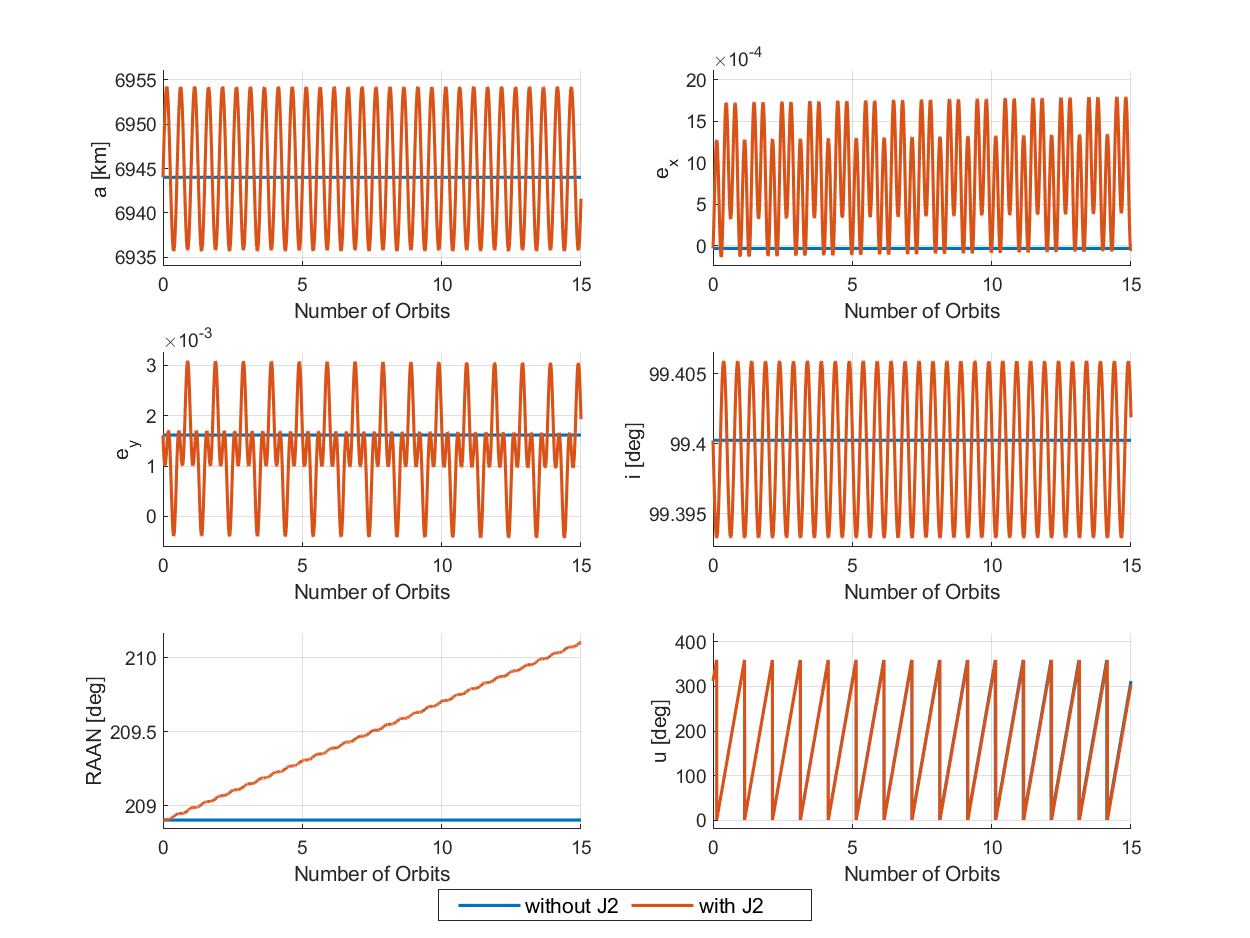
\includegraphics[width=0.75\linewidth]{sim/figures/PS4/OE_abs_osc_SV2.png}
    \caption{Osculating quasi-non-singular orbital elements}
    \label{fig:osc_OE}
\end{figure}

\begin{figure}[H]
    \centering
    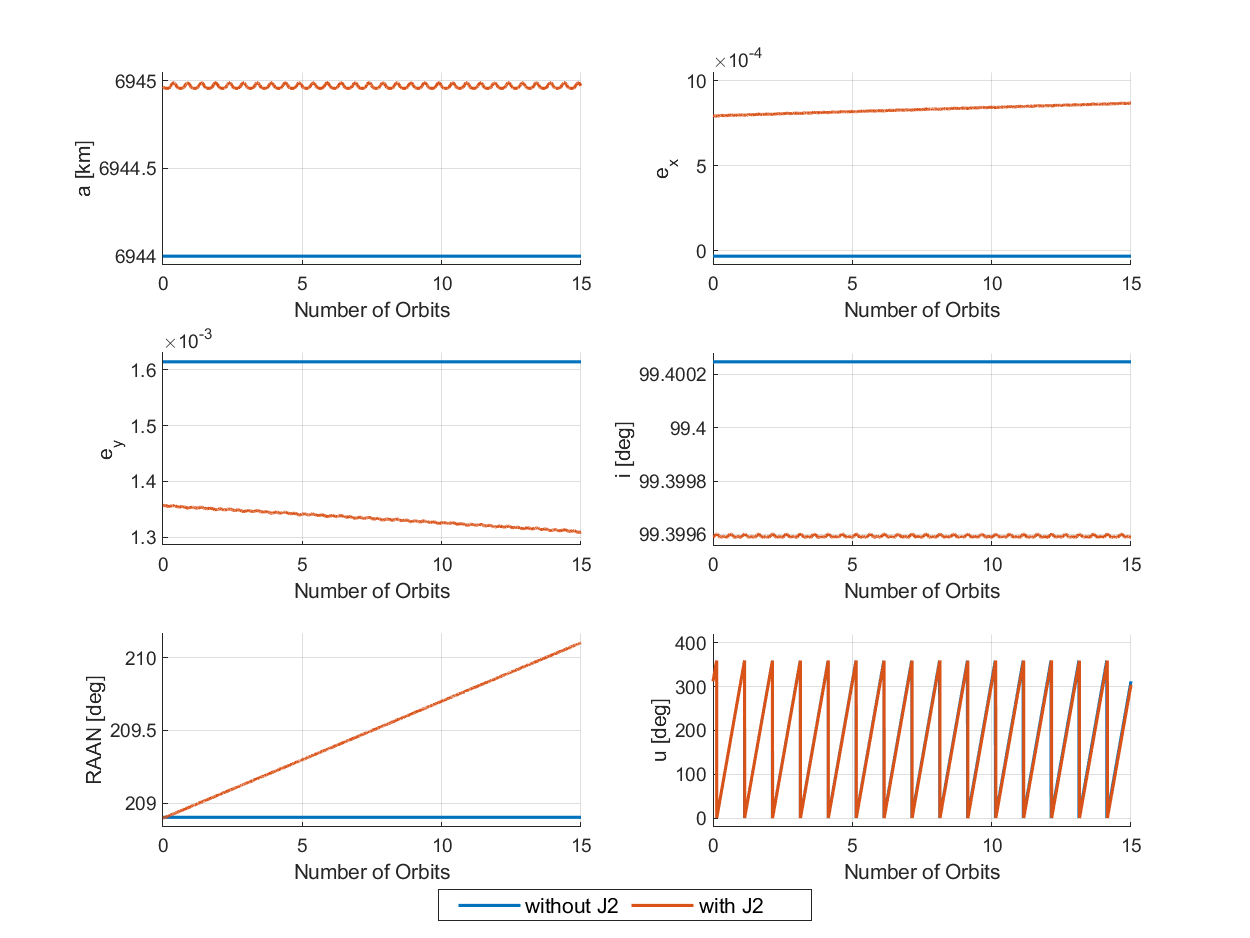
\includegraphics[width=0.75\linewidth]{sim/figures/PS4/OE_abs_mean_SV2.png}
    \caption{Mean quasi-non-singular orbital elements}
    \label{fig:mean_OE}
\end{figure}

\begin{figure}[H]
    \centering
    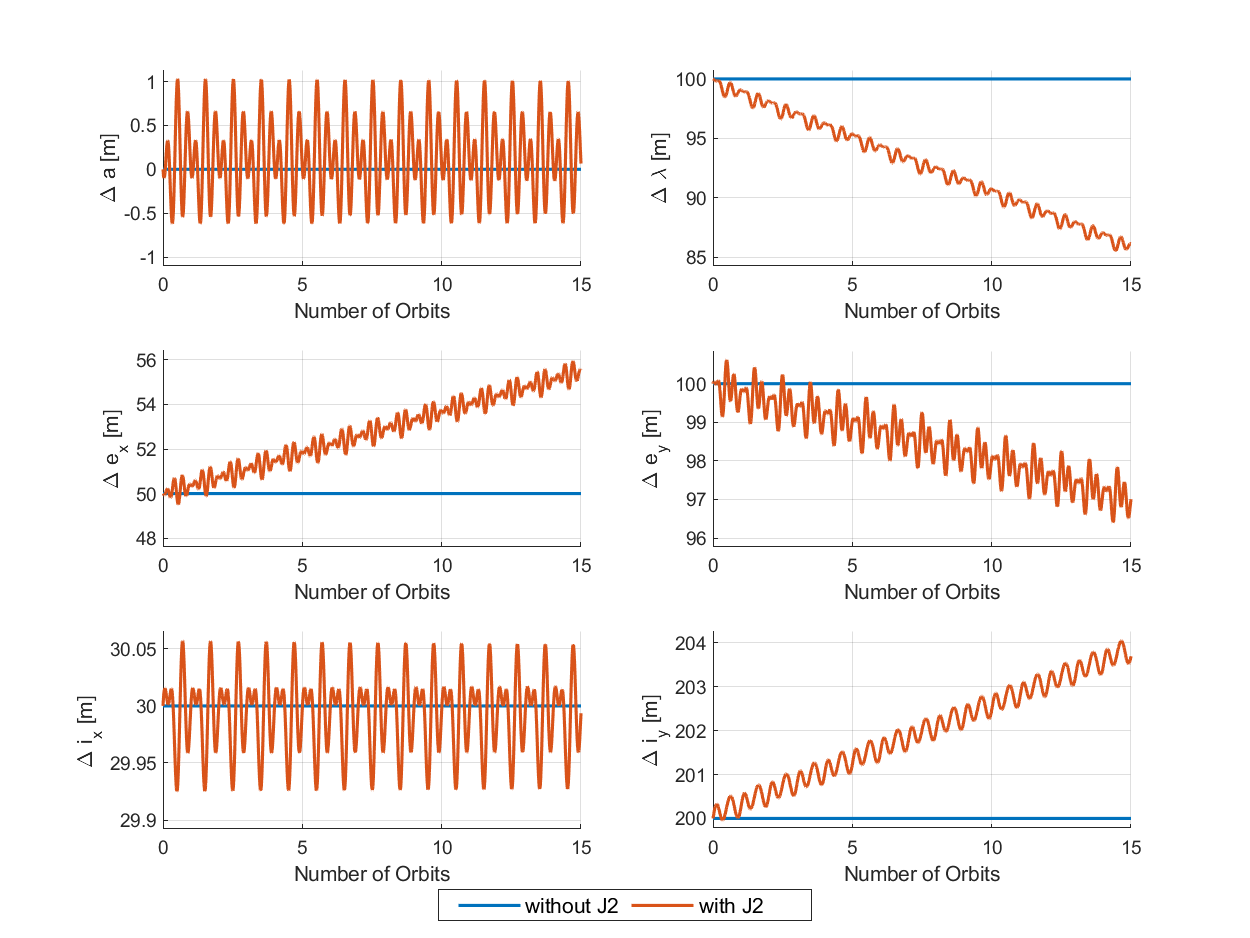
\includegraphics[width=0.75\linewidth]{sim/figures/PS4/ROE_osc_SV2.png}
    \caption{Osculating relative quasi-non-singular orbital elements}
    \label{fig:osc_ROE}
\end{figure}

\begin{figure}[H]
    \centering
    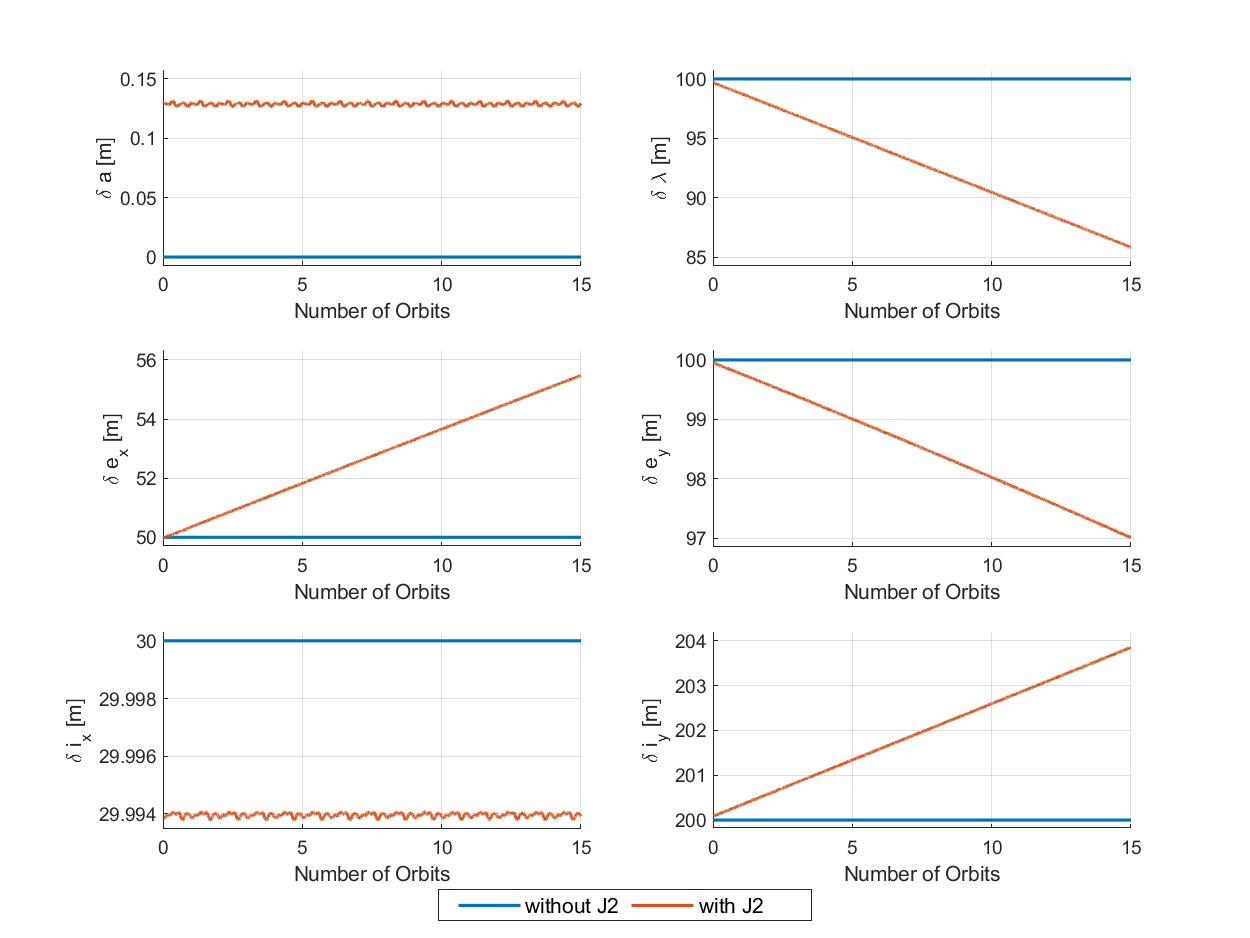
\includegraphics[width=0.75\linewidth]{sim/figures/PS4/ROE_mean_SV2.png}
    \caption{Mean relative quasi-non-singular orbital elements}
    \label{fig:mean_ROE}
\end{figure}

\subsubsection{J2 perturbations in RTN Frame}\label{sec:J2_RTN_frame}
The relative position can also be plotted in the RTN frame. Figure \ref{fig:RTN_3D} shows the relative position in the 3D RTN frame. Figure \ref{fig:RTN_projections} shows the relative position projected into the RTN planes.

\begin{figure}[H]
    \centering
    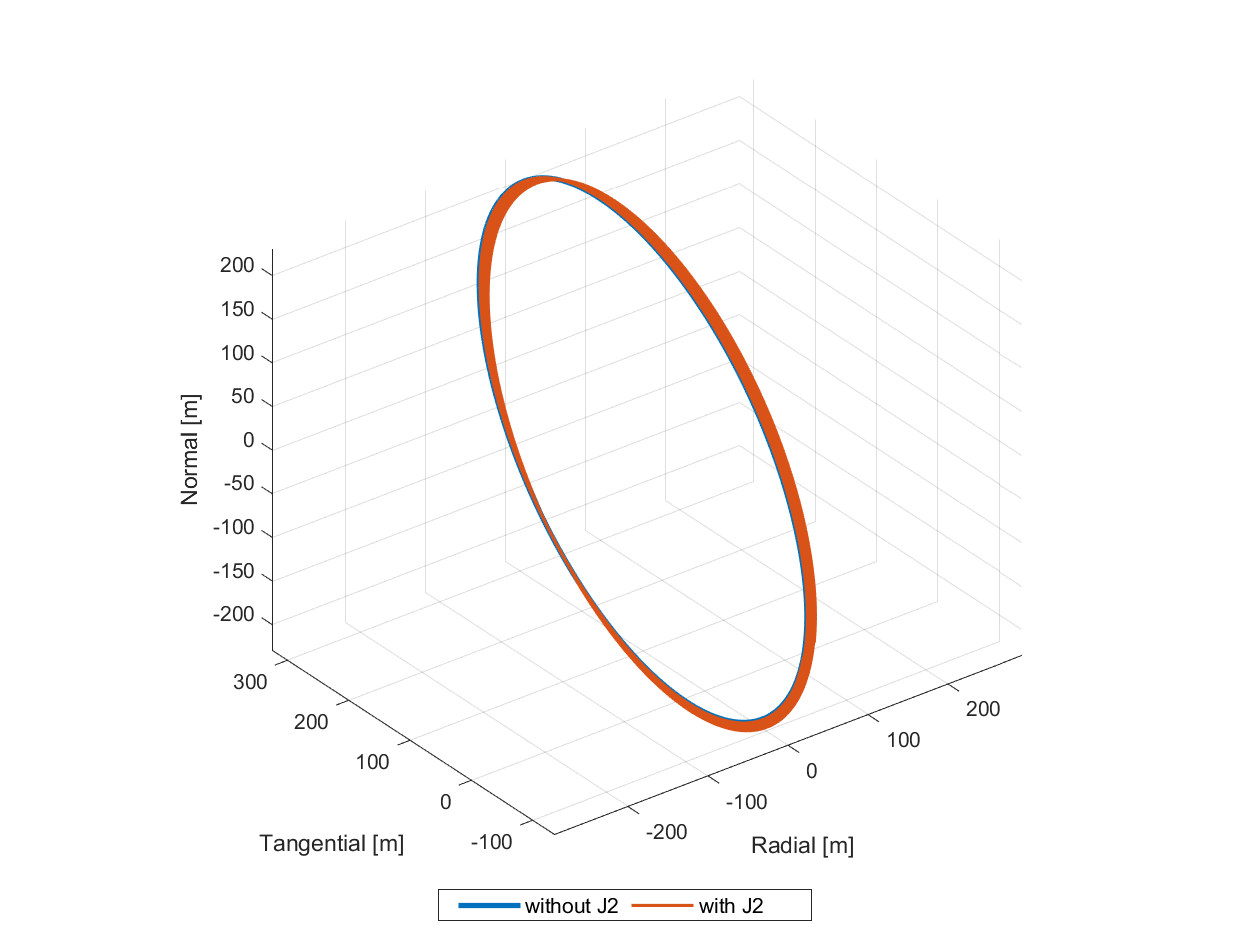
\includegraphics[width=0.75\linewidth]{sim/figures/PS4/RTN_3D_SV2.png}
    \caption{Relative position in RTN 3D}
    \label{fig:RTN_3D}
\end{figure}

\begin{figure}[H]
    \centering
    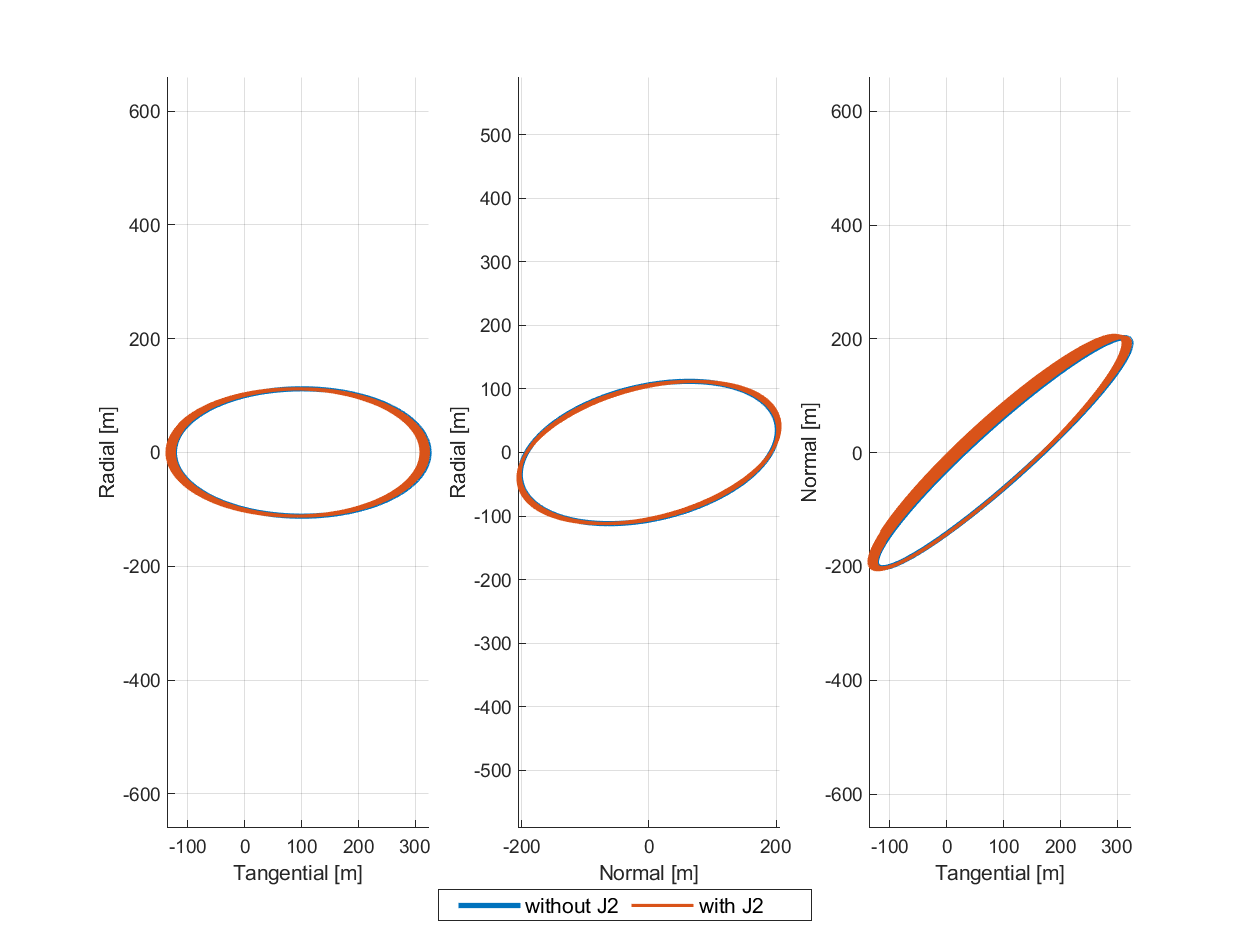
\includegraphics[width=0.75\linewidth]{sim/figures/PS4/RTN_projections_SV2.png}
    \caption{Relative position in RTN projections}
    \label{fig:RTN_projections}
\end{figure}

To understand whether the results are according to our expectations, we need to understand how the relative orbit geometry relates to relative orbital elements. Figure \ref{fig:rel_geometry} shows a figure from the lecture slides. From this, we can see that $\delta a$ determines the center of the relative motion ellipse in the radial direction. $\delta \lambda$ determines the center of the relative motion ellipse in the tangential direction. $\delta e$, which is the L2 norm of $\delta e_x$ and $\delta e_y$, determines the size of this ellipse in the tangential and radial directions. $\delta i$, which is the L2 norm of $\delta i_x$ and $\delta i_y$, determines the size of the ellipse in the normal direction. 

\begin{figure}[H]
    \centering
    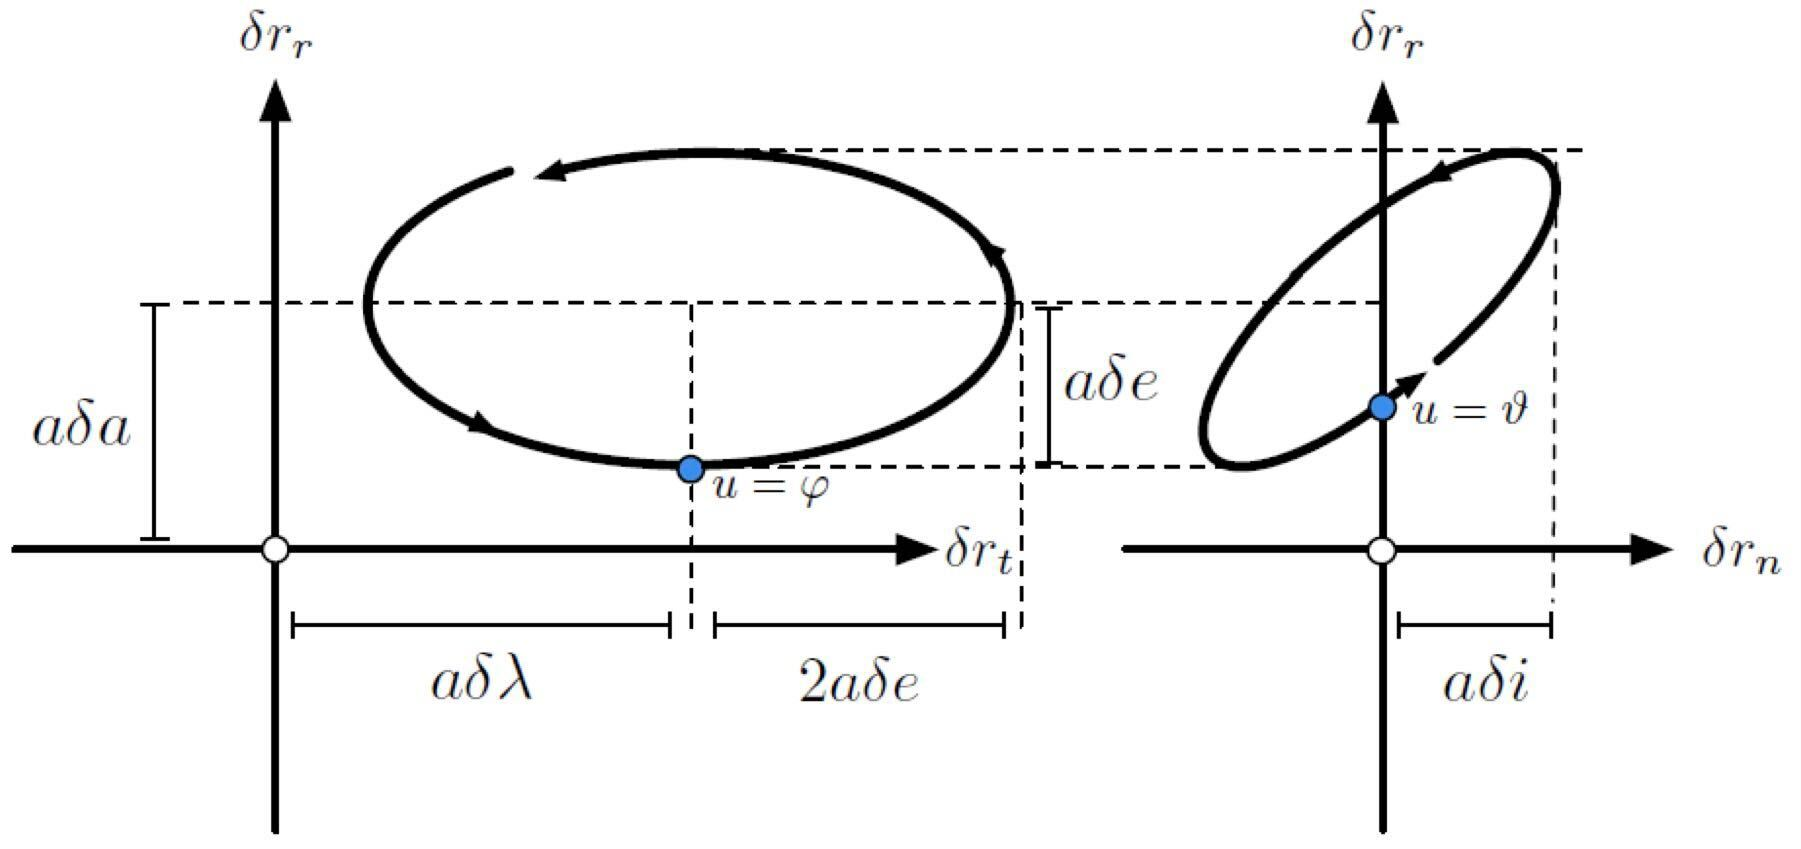
\includegraphics[width=0.75\linewidth]{LaTeX/Figures/RelOrbitGeometry.jpg}
    \caption{Relative orbit geometry}
    \label{fig:rel_geometry}
\end{figure}

Now with that understanding, we look at the effects of J2 on the relative orbital elements. In the quasi-nonsingular relative orbital elements, there are drifts seen in the eccentricity vector $\delta e$, the inclination vector $\delta i$ (specifically the y-component $\delta i_y$), and the mean longitude $\delta \lambda$. The differential J2 effects for near-circular orbits are given by:
\begin{align}
    \frac{d \varphi}{d u} &= \frac{3}{2} \gamma (5\cos^2(i_c) - 1) \\
    \frac{d \delta i_y}{d u} &= 3\gamma \sin^2(i_c) \delta i_x \label{eq:drift_in_rel_i} \\
    \frac{d \delta \lambda}{d u} &= -\frac{21}{2}\left(\gamma \sin(2i_c)\delta i_x 
+ \frac{1}{7} \delta a\right) \label{eq:drift_in_lambda_rel}\\
    \text{where} \quad \gamma  &= \frac{J_2 R_E^2}{2 a^2 (1 - e)^2}
\end{align}
Here, the $\varphi$ is the angle of the eccentricity vector $\delta e$, i.e. $\varphi = \tan^{-1}\left(\frac{\delta e_y}{\delta e_x}\right)$.

Thus, based on these equations and our initial ROE ($\delta a = 0$, $\delta i_x \neq 0$), we expect drifts $\delta i$ and $\delta \lambda$, but not in the magnitude $\delta e$, since only the phase of the relative eccentricity vector is changing, not the magnitude. $\delta i$ has a drift, because J2 only effects the $\delta i_y$ component of the relative inclination vector. From the drift in $\delta \lambda$, we expect to see a drift of the ellipse in the tangential direction in the RTN frame, which is observed. From the drift in the phase of $\delta e$, we expect to see the ellipse starting to rotate as its "relative perigee" drifts circularly. This too is observed in the RTN frame. Thus, the results in the RTN frame are as expected given the initial relative orbital elements. Finally, from the drift in $\delta i$ we expect to see a drift of the ellipse in the normal direction in the RTN frame, which, while not very significant, is also observed. 


\subsubsection{J2 perturbations in ROE space}
The osculating and mean quasi-non-singular orbital elements can be plotted in a different way to better examine their behavior with and without J2, as shown in Figure \ref{fig:osc_ROE_proj} and Figure \ref{fig:mean_ROE_proj}. Again, the osculating and mean results line up well for the secular drifts, with the osculating also showing short-term periodic behavior. 

\begin{figure}[H]
    \centering
    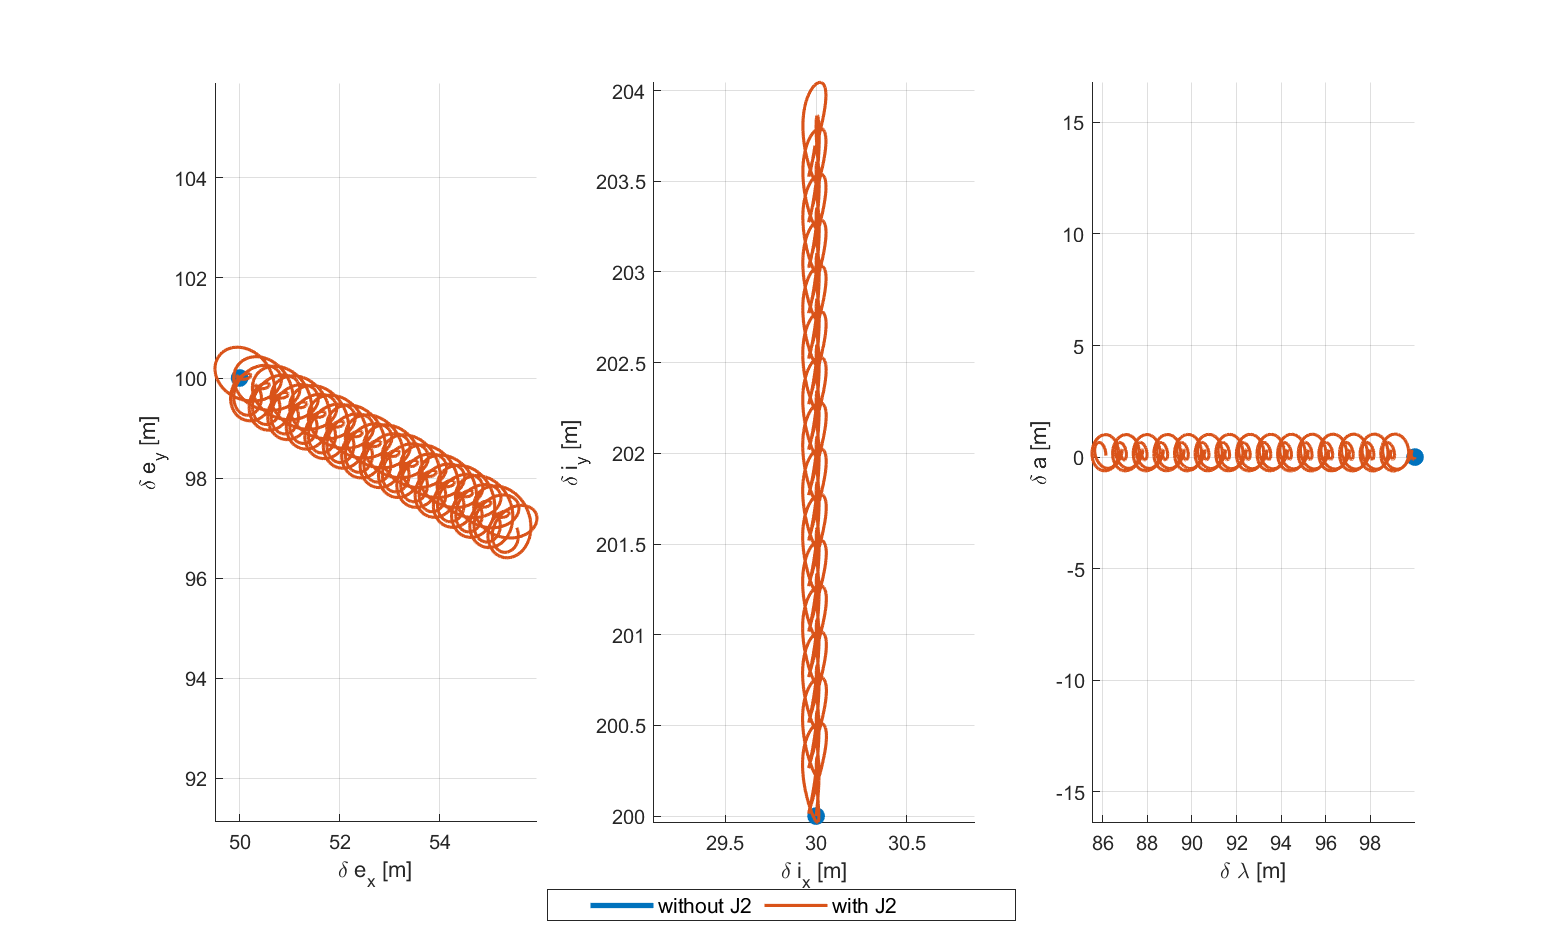
\includegraphics[width=0.75\linewidth]{sim/figures/PS4/ROE_projections_osc_SV2.png}
    \caption{Osculating relative quasi-non-singular orbital elements}
    \label{fig:osc_ROE_proj}
\end{figure}
\begin{figure}[H]
    \centering
    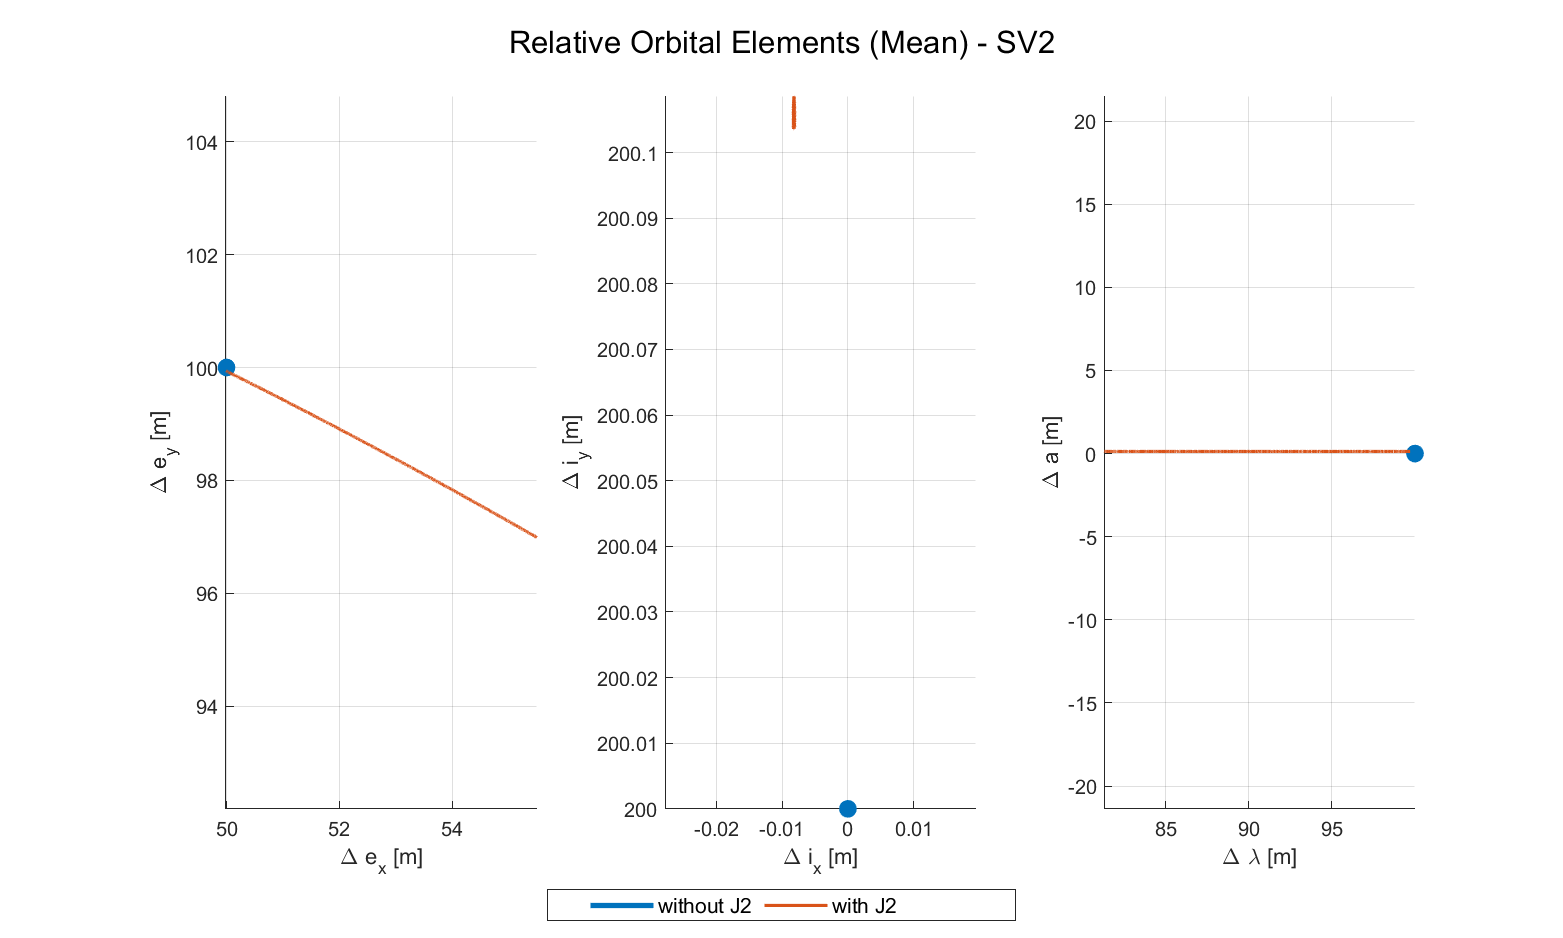
\includegraphics[width=0.75\linewidth]{sim/figures/PS4/ROE_projections_mean_SV2.png}
    \caption{Mean relative quasi-non-singular orbital elements}
    \label{fig:mean_ROE_proj}
\end{figure}

These results line up with the behavior observed in the relative position in RTN and as preidted from the initial relative orbital elements. As discussed in the previous section, the eccentricity vector is starting to trace out a circle as its phase drifts. Only a small part of this circle is observed here because we simulated for 15 orbits or about 1 day, while it takes 100-200 days to complete the full rotation in phase. The drift in $\delta i_y$ matches the drift in the normal direction in RTN observed previously and matches the governing equations in the previous section. The drift in $\delta \lambda$ is dependent on $\delta a$ and $\delta i_x$. The drift from $\detla_a$ is referred to as the Keplerian drift while the component from $\delta i_x$ arises from J2. The Keplerian drift leads to a decreasing or increasing $\delta \lambda$ depending on the sign of $\delta a$, while the J2 drift acts in the opposite direction. However, the Keplerian drift is significantly larger in magnitude with a non-zero $\delta a$. Although our initial $\delta a$ is 0, once we propagate with J2, we observe a non-zero $\delta a$ in osculating and mean elements. This issue is addressed in later problem sets to ensure that a non-zero $\delta a$ does not persist. Nonetheless, for this problem set, the non-zero $\delta a$ is why we observe a drift in the decreasing $\delta \lambda$ direction. This drift is a combination of the larger Keplerian drift from non-zero $\delta a$ and the smaller J2 drift (in the opposite direction) from non-zero $\delta i_x$.

\subsubsection{Maneuver to remove J2 secular effects}\label{sec:J2_maneuver}
From the equations in Section \ref{sec:J2_RTN_frame}, we see that the drift in the eccentricity vector is periodic circular rather than secular. Therefore, to eliminate the secular drift we just need to eliminate the secular effects in the inclination vector and the mean longitude. The circular periodic drift in the eccentricity could also be eliminated by choosing a critical inclination for the deputy. 

From Equation \ref{eq:drift_in_rel_i}, we see that one way to remove this differential effect in the inclination vector is by setting $\delta i_x = 0$. From Equation \ref{eq:quasi_nonsign_roe}, $\delta i_x = 0 \implies i_t = i_o$, or in other words the deputy satellite and the chief satellite have the same orbital inclination. 

To completely remove the drift in the mean longitude based on Equation \ref{eq:drift_in_lambda_rel}, we would need to not only set $\delta i_x = 0$ but also  $\delta a = 0$. Although Equation \ref{eq:drift_in_lambda_rel} only shows the Keplerian drift caused by $\delta a$, there is also a component of J2 drift that is a result of a non-zero $\delta a$ (not shown here, but is implied by the state-transition matrix provided in \cite{koenig2017new} and Section \ref{sec:j2_analytical_roe}. 

Based on the given initial conditions in Section \ref{sec:ic_for_pset4}, we assume that the $\delta a = 0$ already. So the maneuver would mainly be to remove the inclination difference. We will see in following sections that the $\delta a = 0$ assumption does not hold over al time for our case, and that even after setting $\delta i_x = 0$, we see a drift in $\delta \lambda$.

The optimal location (minimum $\Delta v$) to produce an orbital inclination change is at the line of nodes of the orbit, i.e. when $u_M = 0^\circ \ \text{or} \ 180^\circ$. The maneuver should be normal to the orbital plane, and the magnitude of the $\Delta v$ is given by
\begin{align}
    \Delta v_M = 2v\sin\left(\frac{i_t - i_o}{2}\right)
\end{align}

For near-circular, we can take $v = \sqrt{\frac{\mu}{a}} = na$, we get

\begin{align}
    \Delta v_M = 2na_c\sin\left(\frac{i_t - i_o}{2}\right)
\end{align}

Using the properties of the chief's orbit and a $\Delta i = 30 m/a_c = 1.237\cdot 10^{-4}$ degrees, we get

\begin{align}
    \Delta v_M = 3.27 \cdot10^{-2} \ m/s
\end{align}

\subsubsection{Simulation with new initial conditions that don't have secular effects}

We set the initial condition $\delta i_x = 0$ to remove secular effects. With this, we get the relative orbital elements over time shown in Figure \ref{fig:rel_roe_no_drift_mean} (mean ROE) and \ref{fig:rel_roe_no_drift_osc} (osculating ROE).

\begin{figure}[H]
    \centering
    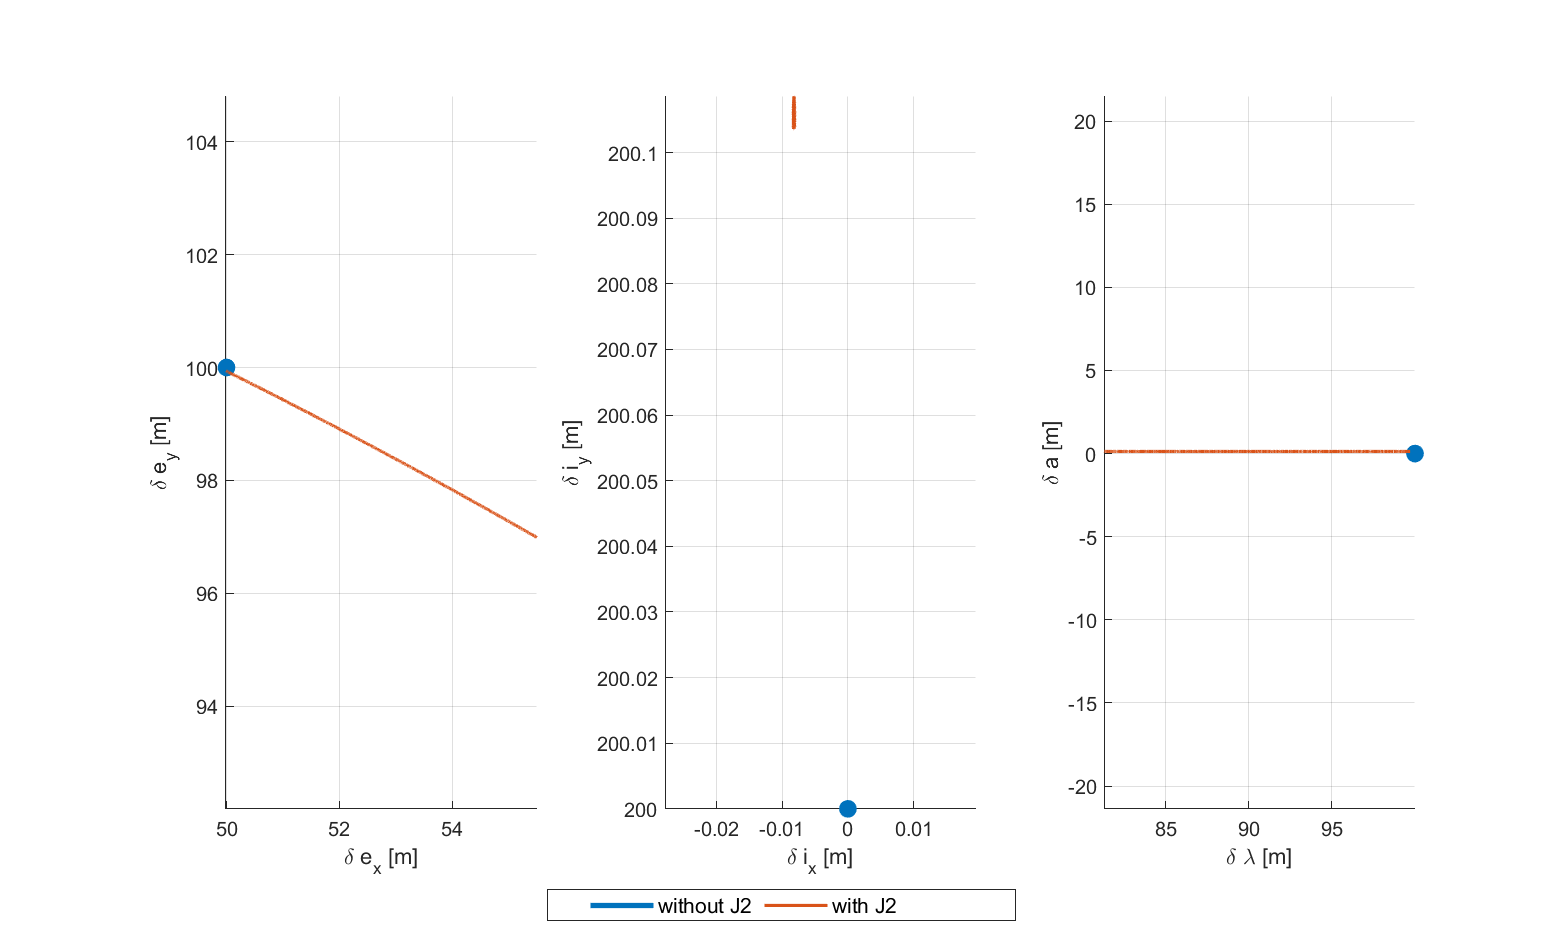
\includegraphics[width=0.8\linewidth]{sim/figures/PS4/ROE_projections_mean_no_drift_SV2.png}
    \caption{Relative mean orbital elements with initial conditions set to remove the secular effects. Note that the $\delta i_y$ axis has small bounds.}
    \label{fig:rel_roe_no_drift_mean}
\end{figure}

\begin{figure}[H]
    \centering
    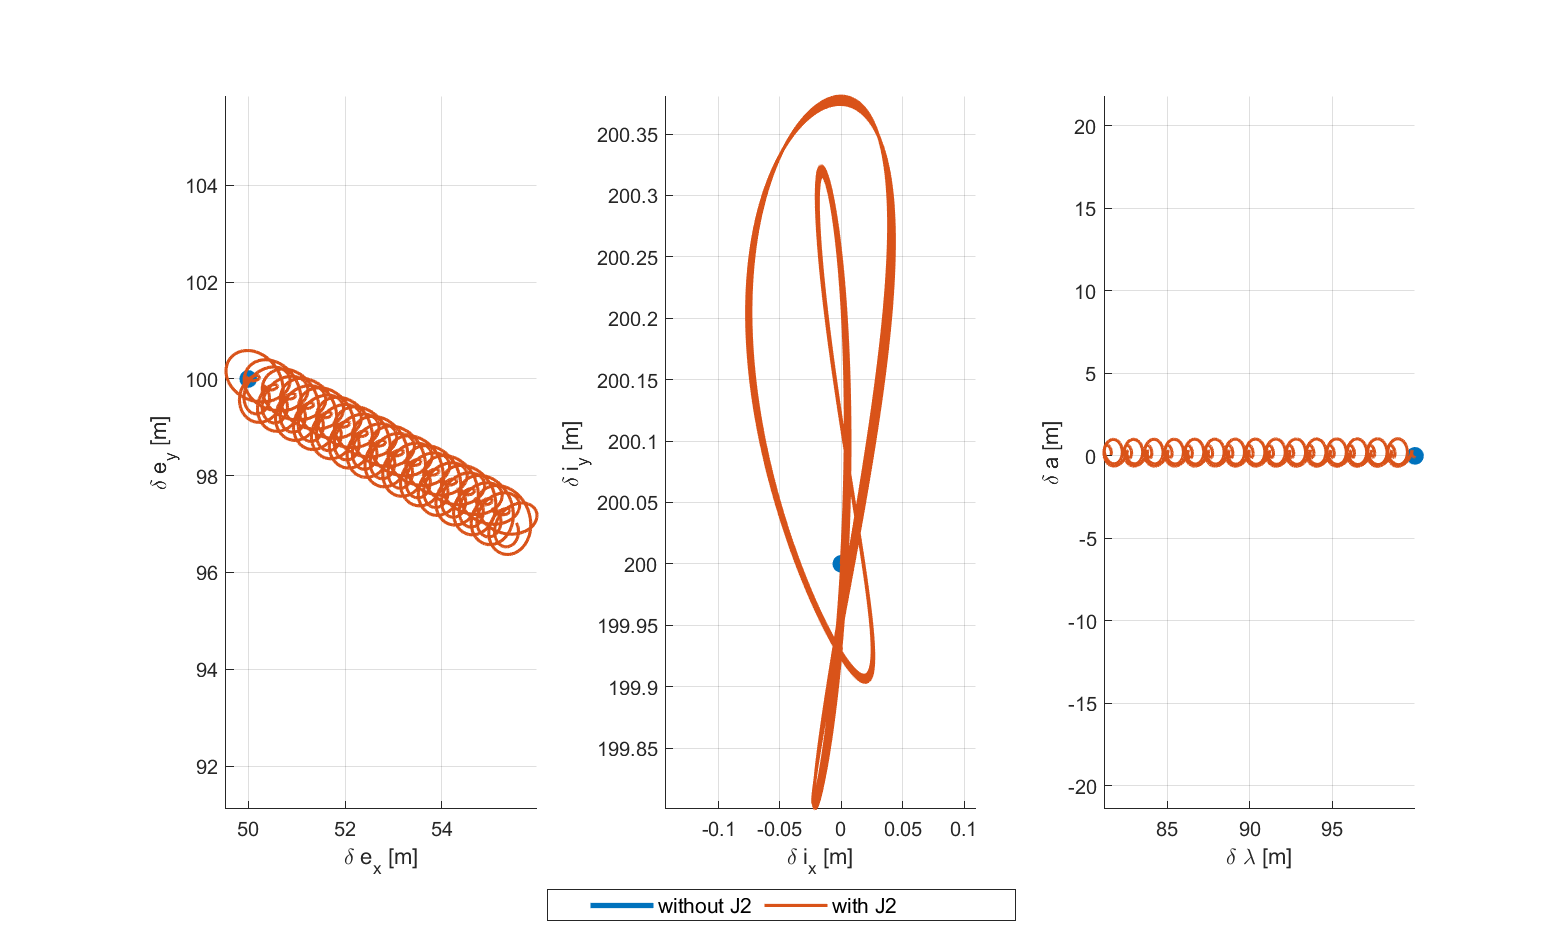
\includegraphics[width=0.8\linewidth]{sim/figures/PS4/ROE_projections_osc_no_drift_SV2.png}
    \caption{Relative osculating orbital elements with initial conditions set to remove the secular effects. Note that the $\delta i_y$ axis has small bounds.}
    \label{fig:rel_roe_no_drift_osc}
\end{figure}

We see that there are a few differences when comparing these to the osculating orbital elements seen in Figure \ref{fig:osc_ROE_proj} and the mean orbital elements seen in \ref{fig:mean_ROE_proj}. Specifically, the drift in the $\delta i_y$ is significantly smaller, with any remaining error attributed to numerical error. Second, we see that the drift in $\delta \lambda$ was not removed, and in fact increased in drift compared to Figure \ref{fig:mean_ROE_proj}. This is because, although the J2 effects related to inclination have been removed, there is still non-zero $\delta a$ during propagation (this is easy to see in the mean $\delta a$ plot in Figure \ref{fig:mean_ROE}), and this causes both J2 drift and a Keplerian drift. Additional control would be needed to remove this additional $\delta a$ difference during propagation.

\subsubsection{Analytical Solution for J2 on Relative Orbital Elements} \label{sec:j2_analytical_roe}

By taking a first-order approximation of the equations of motion for the relative orbital elements with J2 perturbations included, we can derive a state transition matrix that is completely based on the absolute orbital parameters of the chief satellite \cite{koenig2017new}. Then the relative orbit parameter set $\boldsymbol{\alpha}$ at any time $\tau$ can be found using
\begin{align}
    \boldsymbol{\alpha_{\tau}} = \Phi^{J_2}_{\text{qns}}(\alpha_c(t_i), \tau) \boldsymbol{\alpha_{i}} \label{eq:state_transition_relation}
\end{align}

where $\Phi^{J_2}_{\text{qns}}(\alpha_c(t_i), \tau)$ is the state-transition matrix (STM) at time $\tau$, and $\boldsymbol{\alpha_{i}}$ are the initial conditions of the relative orbital elements.

The state-transition matrix for quasi-nonsingular relative orbital elements is given by
\begin{align}
&\Phi^{J_2}_{\text{qns}}(\alpha_c(t_i), \tau) = \nonumber \\ 
&\begin{bmatrix}
1 & 0 & 0 & 0 & 0 & 0 \\
-\left( \frac{3}{2}n + \frac{7}{2} \kappa E P \right)\tau & 1 & \kappa e_{x_i} F G P \tau & \kappa e_{y_i} F G P \tau & -\kappa F S \tau & 0 \\
\frac{7}{2} \kappa e_{y_f} Q \tau & 0 & \cos(\dot{\omega} \tau) - 4\kappa e_{x_i} e_{y_f} G Q \tau & -\sin(\dot{\omega} \tau) - 4\kappa e_{y_i} e_{y_f} G Q \tau & 5\kappa e_{y_f} S \tau & 0 \\
-\frac{7}{2} \kappa e_{x_f} Q \tau & 0 & \sin(\dot{\omega} \tau) + 4\kappa e_{x_i} e_{x_f} G Q \tau & \cos(\dot{\omega} \tau) + 4\kappa e_{y_i} e_{x_f} G Q \tau & -5\kappa e_{x_f} S \tau & 0 \\
0 & 0 & 0 & 0 & 1 & 0 \\
\frac{7}{2} \kappa S \tau & 0 & -4 \kappa e_{x_i} G S \tau & -4 \kappa e_{y_i} G S \tau & 2 \kappa T \tau & 1
\end{bmatrix} \label{eq:stm_matrix}
\end{align}

where we have the following variables
\begin{align*}
\eta &= \sqrt{1 - e^2} &
\kappa &= \frac{3}{4} \frac{J_2 R_E^2 \sqrt{\mu}}{a^{7/2} \eta^4} &
E &= 1 + \eta \\
F &= 4 + 3\eta &
G &= \frac{1}{\eta^2} & \\
P &= 3\cos^2(i) - 1 &
Q &= 5\cos^2(i) - 1 &
R &= \cos(i) \\
S &= \sin(2i) &
T &= \sin^2(i) &
U &= \sin(i) \\
V &= \tan(i/2) &
W &= \cos^2(i/2)
\end{align*} 

We first apply this to the initial conditions described in Section \ref{sec:ic_for_pset4} where $\delta i_x \neq 0$.
It is important to note here that the analytical state transition matrix is a result of making first-order approximations (including the assumption that $\delta a$ remains constant). Therefore, this analytical result does not capture osculation behavior caused by J2 perturbations. If we just use the osculating initial conditions specified in Section \ref{sec:ic_for_pset4}, we get the result in Figure \ref{fig:roe_analytical_compare_osc}. Clearly, the results don't align completely.

\begin{figure}[H]
    \centering
    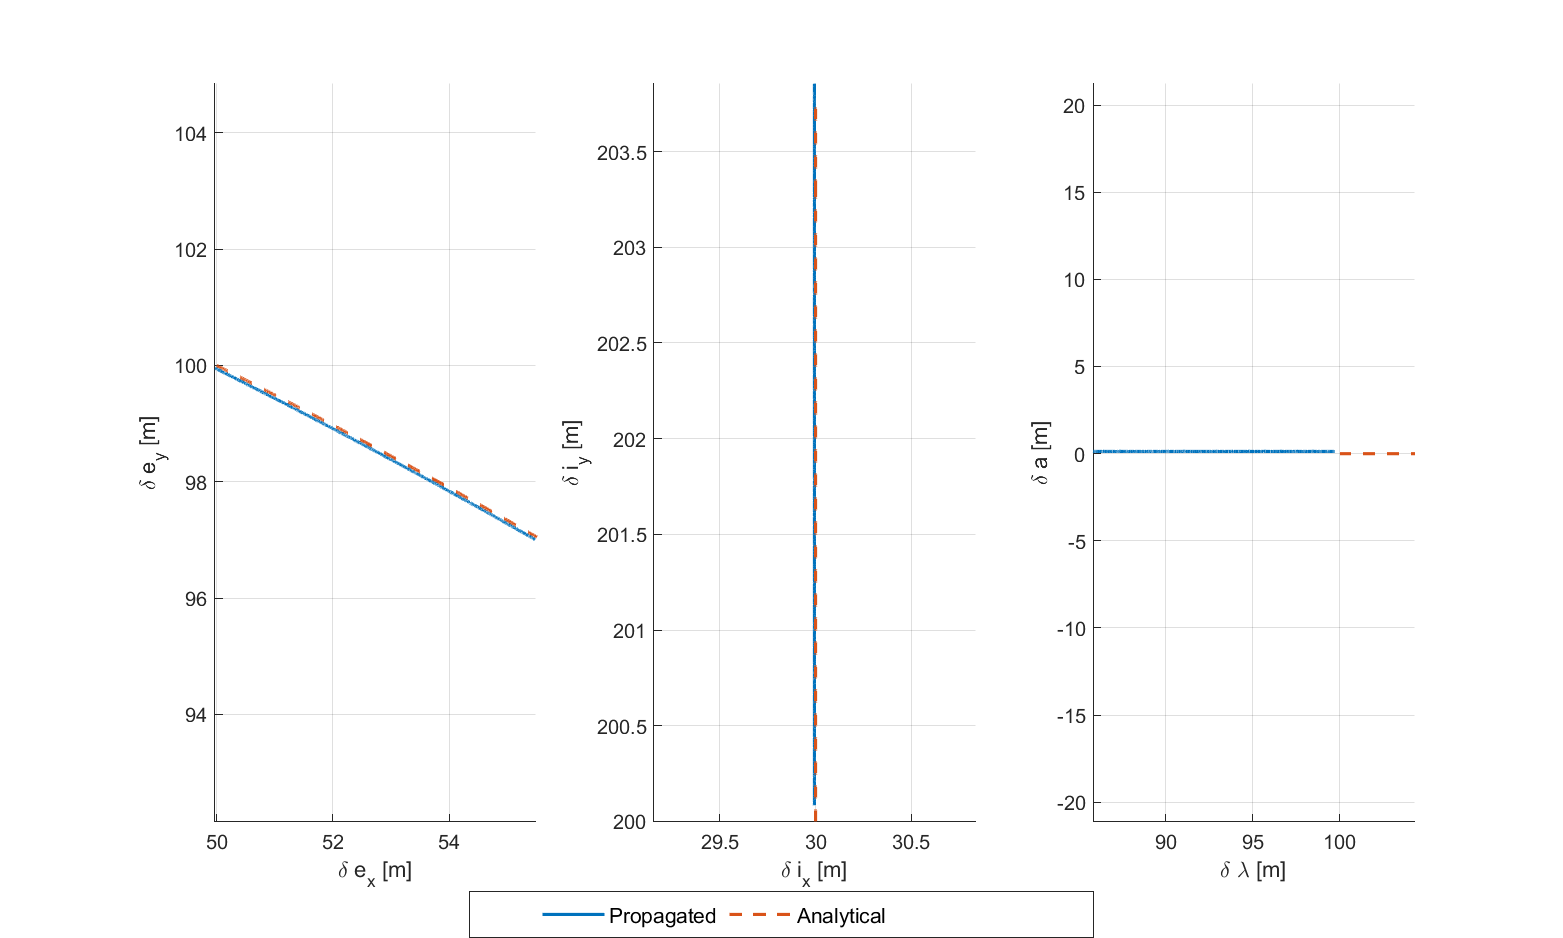
\includegraphics[width=0.8\linewidth]{sim/figures/PS4/ROE_analytical_compare_given_IC2_SV2.png}
    \caption{Comparison of the (mean) propagated and analytical relative orbital elements, using the osculating initial conditions for the analytical result.}
\label{fig:roe_analytical_compare_osc}
\end{figure}

Most noticeable is the divergence in the $\delta \lambda$. The propagated $\delta \lambda$ is in fact going in the opposite direction as the expected $\delta \lambda$ drift due to J2 effects and a zero $\delta a$. This can be attributed to the osculating effects that are not captured in the analytical result. This error is primarily seen in the $\delta \lambda$ plot, although there are also a small offset in the $\delta e$ and $\delta i$ plots.

Now, instead of using the given osculating initial conditions to test our analytical result, we can use the initial conditions converted to mean relative orbital elements. If we now use those when calculating the analytical, we see that the results match much better, as seen in Figure \ref{fig:roe_analytical_compare_mean}. In this case, the $\delta \lambda$ also watches very well.

\begin{figure}[H]
    \centering
    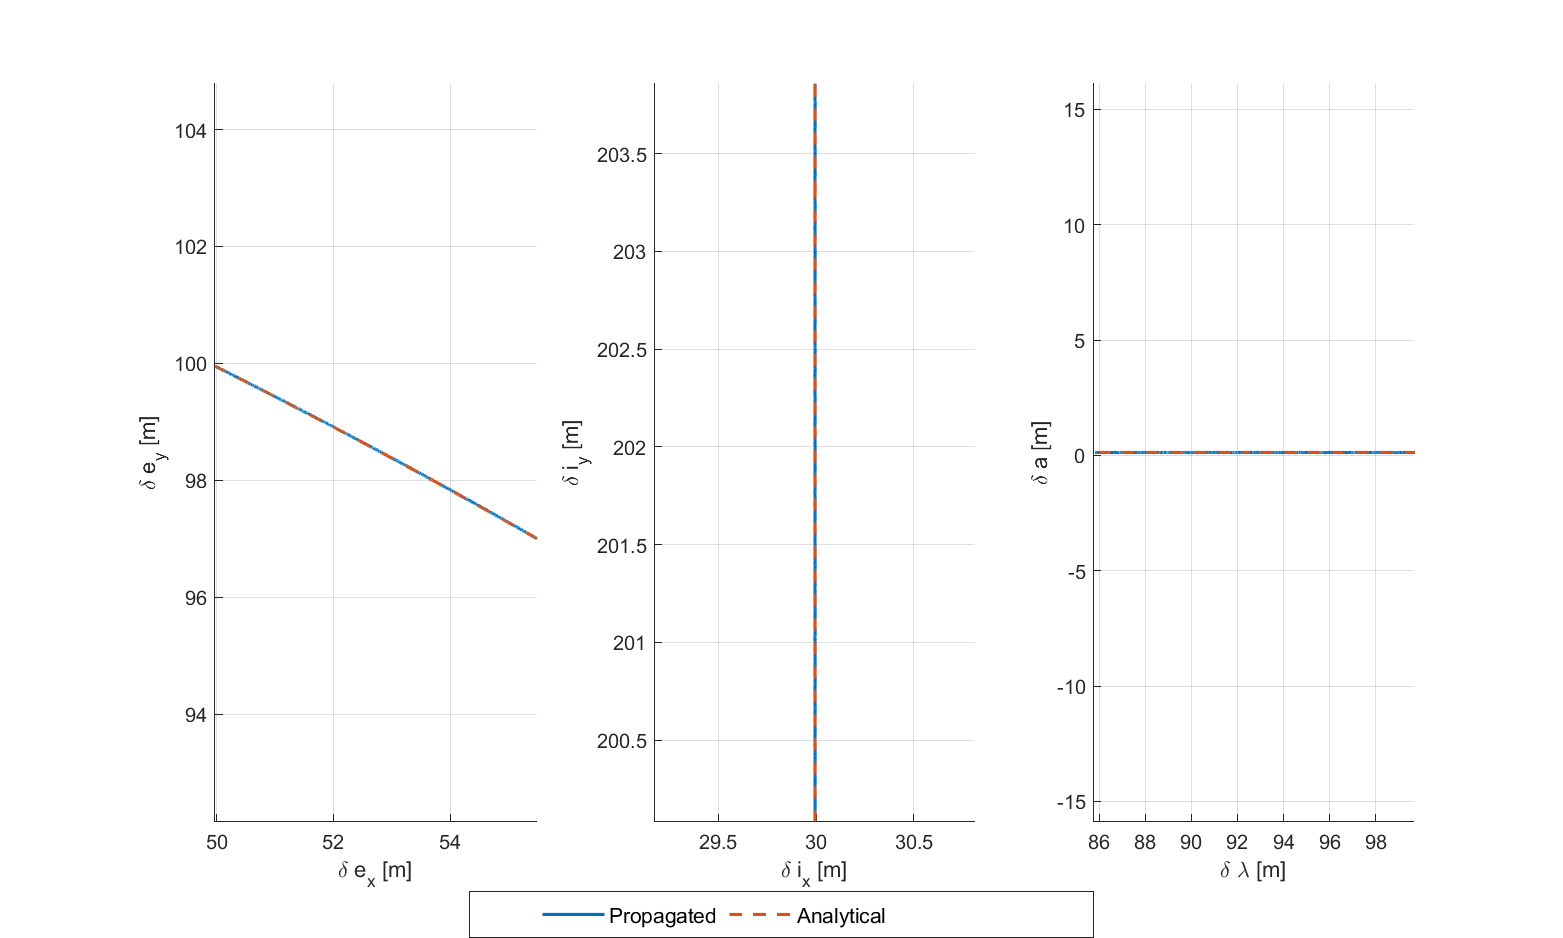
\includegraphics[width=0.8\linewidth]{sim/figures/PS4/ROE_analytical_compare_mean_IC2_SV2.png}
    \caption{Comparison of the propagated and analytical relative orbital elements, but using the mean initial conditions for the analytical result.}
\label{fig:roe_analytical_compare_mean}
\end{figure}

We can similarly also analyze the results from setting the initial conditions to be the set from Section \ref{sec:J2_maneuver}. Figure \ref{fig:roe_analytical_compare_osc_zeroed} is the result of setting the initial conditions to the given osculating values, and Figure \ref{fig:roe_analytical_compare_mean_zeroed} is the result of setting the initial conditions to the mean values. Once again, the result is the same as before where the analytical solution agrees with the propagated result better (including capturing the $\delta \lambda$ drift caused by the non-constant $\delta a$) when we use the mean initial conditions.

\begin{figure}[H]
    \centering
    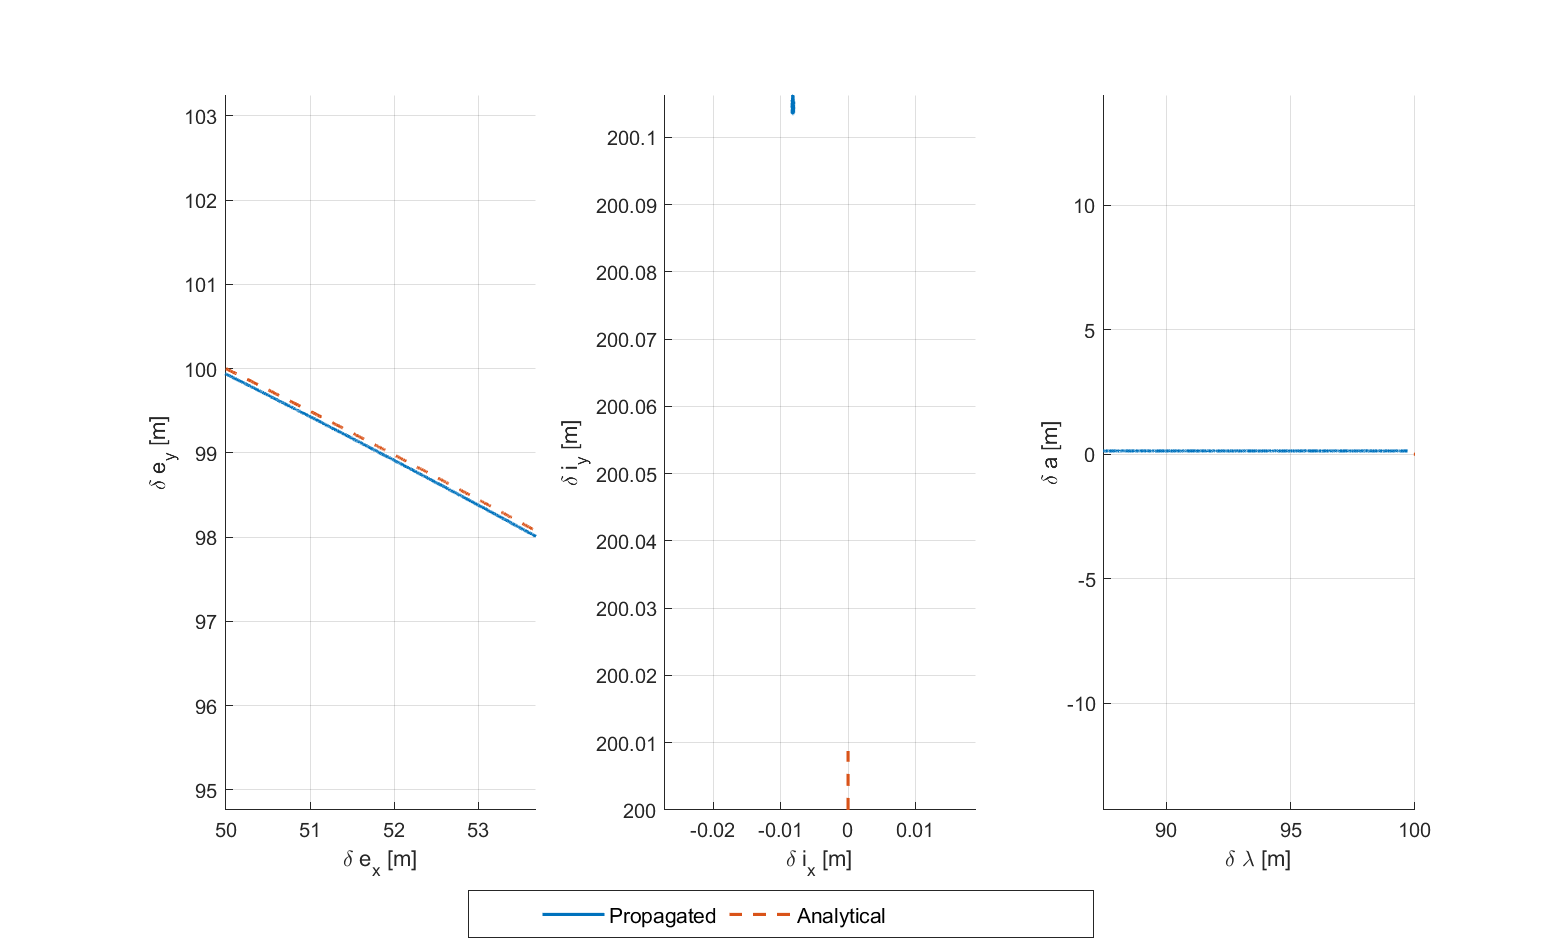
\includegraphics[width=0.8\linewidth]{sim/figures/PS4/ROE_analytical_compare_given_IC3_SV2.png}
    \caption{Comparison of the (mean) propagated and analytical relative orbital elements, using the osculating initial conditions with $\delta i_x = 0$ for the analytical result. Note here that the axes of the inclination vector are small, and that the analytical $\delta \lambda$ shows no propagation.}
\label{fig:roe_analytical_compare_osc_zeroed}
\end{figure}

\begin{figure}[H]
    \centering
    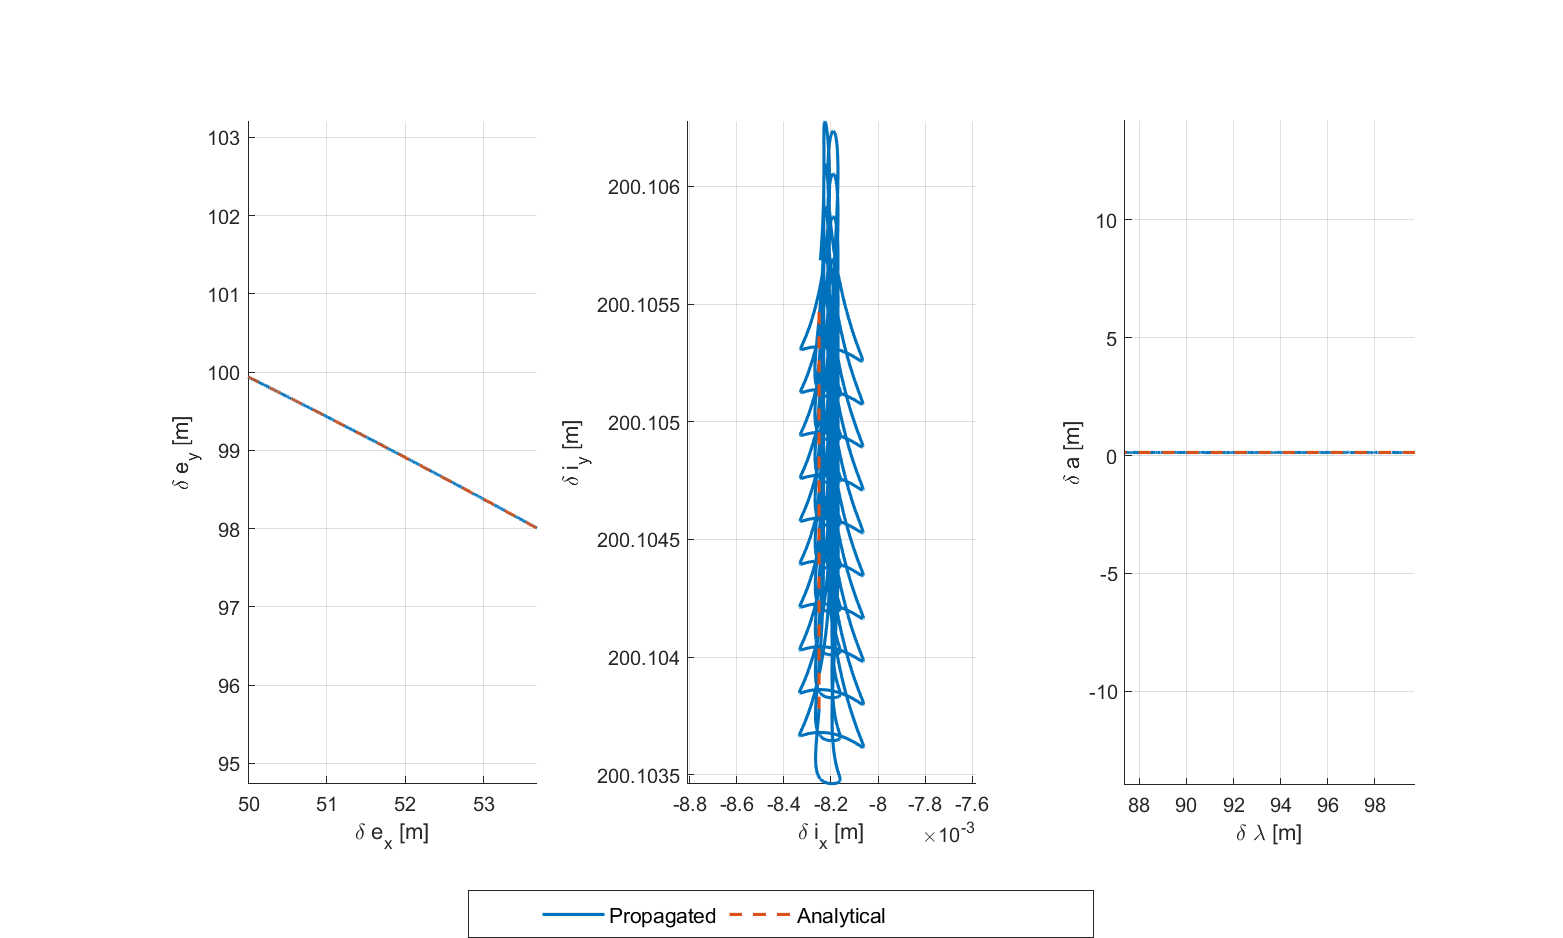
\includegraphics[width=0.8\linewidth]{sim/figures/PS4/ROE_analytical_compare_mean_IC3_SV2.png}
    \caption{Comparison of the (mean) propagated and analytical relative orbital elements, using the mean initial conditions with $\delta i_x = 0$ for the analytical result. Note here that the axes of the inclination vector are small.}
\label{fig:roe_analytical_compare_mean_zeroed}
\end{figure}

The takeaway from this is that there are osculating effects on the relative orbital elements that cannot be ignored, so using mean relative orbital elements initial conditions is required to get the analytical solution to match the propagated mean relative orbital elements result.